\chapter{FUNDAMENTOS TEÓRICOS}

\section{SERIES DE TIEMPO}

Son una secuencia de observaciones refiriéndose a datos que se recopilan y registran en intervalos de tiempo regulares, 
la información se encuentra ordenada cronológicamente por un único identificador de secuencia tanto cronológico como posicional,
el principal objetivo de la series de tiempo, es permitir el análisis de la información procesada para hacer un pronóstico 
de los futuros eventos.

Cuando una serie de tiempo enfoca una unidad observable en diferentes momentos se denomina \textit{Serie Temporal Univariante} y matemáticamente 
se representan de la forma: \\
%\[\boxed{y_1,y_2,...,y_N; {(yt)^N} t=1; (yt : t=1,...,N)}\]
${y_1,y_2,...,y_N; {(yt)^N} t=1; (yt : t=1,...,N)}$, Donde $yt$ es la observación $n^0 t (1 \leq t \leq N)$ de la serie y $N$ es el número de observaciones de que 
consta la serie completa. Las $N$ observaciones $y_1,y_2,...,y_N$ pueden recogerse en un vector columna $Y \equiv [y_1,y_2,...,y_N]$ de orden $Nx1$

Sí en una serie de tiempo enfoca varias unidades observables en diferentes momentos se denomina \textit{Serie Temporal Multivariante} y frecuentemente se la puede 
encontrar representada de la forma: \\
${Y_1,Y_2,...,Y_N; {(Yt)^N} t=1; (Yt : t=1,...,N)}$, donde $Y \equiv [Y_1,Y_2,...,Y_N]$ ($M\geq2$) es la observación $n^0 t (1 \leq t \leq N)$ de la serie 
y $N$ es el número de observaciones de que consta la serie completa,las $N$ observaciones $Y_1,Y_2,...,Y_N$ pueden recogerse en una matriz $Y$ de orden $MxN$
\begin{gather*}
Y \equiv
\begin{bmatrix}
Y_1' \\
y_2' \\
\vdots \\
Y_N' \\
\end{bmatrix}
\equiv
\begin{bmatrix}
y_{11} & y_{12} & ... & y_{1M} \\
y_{21} & y_{22} & ... & y_{2M} \\
\vdots & \vdots & \vdots & \vdots \\
y_{N1} & y_{N2} & ... & y_{NM} \\
\end{bmatrix}
\\
\end{gather*}
Donde $Y_{tj}$ es la observación $n^0$ tal que $t (1 \leq t \leq N)$ sobre la característica o variable $N^0$ tal que $j(1 \leq t \leq N)$, que es la misma 
en todo momento $t$.\\

\subsection{Componentes}

los componentes más comunes en las series de tiempo están directamente relacionados con la variación de las observaciones, observaciones que al 
sobreponerse o actuar en concierto, contribuyen a los cambios observados en un período de tiempo y dan a la serie su tendencia, aspecto errático, entre los
componentes mas comunes encontramos: 
\begin{itemize}
  \item{\textbf{Tendencia secular}}: también denominada tendencia a largo plazo de una serie, es por lo común el resultado de factores a largo plazo. 
  En términos intuitivos, la tendencia de una serie de tiempo caracteriza el patrón gradual y consistente de las variaciones de la propia serie, que 
  se consideran consecuencias de fuerzas persistentes que afectan el crecimiento o la reducción de la misma. Las tendencias a largo plazo se ajustan a 
  diversos esquemas. Algunas se mueven continuamente hacía arriba, otras declinan, y otras más permanecen igual en un cierto período o intervalo de tiempo.
  \begin{figure}[htb]
    \centering 
    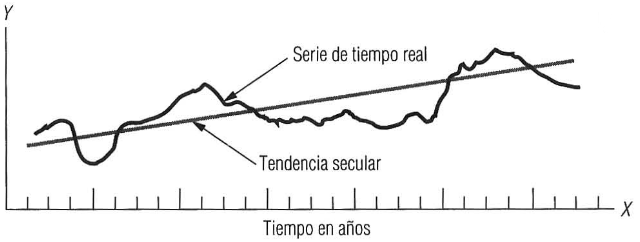
\includegraphics[width=0.7\textwidth]{pictures/tsc1.png}
    \caption{Representación de Tendencia secular en una serie de tiempo}
    \label{fig:tsc1}
  \end{figure}
  
  \item{\textbf{Variación estacional}}: comprende la representación de la variabilidad en los datos debida a influencias de las estaciones. Esta variación
  corresponde a los movimientos de la serie que recurren año tras año en los mismos meses del año poco más o menos con la misma intensidad. Este tipo de variación
  implica patrones de cambio en el lapso de un ano que tienden a repetirse anualmente. Por ejemplo, un médico puede esperar un aumento sustancial en el número de 
  casos de gripe cada invierno y de afectados de tifoidea cada verano. Como se trata de patrones regulares son útiles al pronosticar el futuro. La Figura ~\ref{fig:tsc2} 
  muestra la variación estacional, se puede notar como la serie de tiempo alcanza un pico cada cuarto trimestre del año.
  \begin{figure}[htb]
    \centering 
    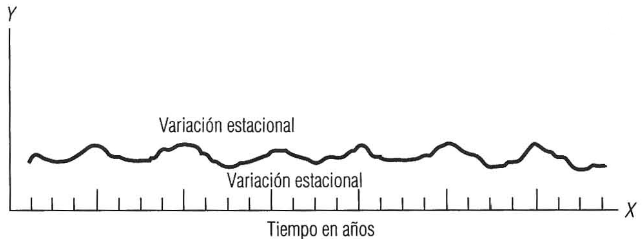
\includegraphics[width=0.7\textwidth]{pictures/tsc2.png}
    \caption{Representación de Variación estacional en una serie de tiempo}
    \label{fig:tsc2}
  \end{figure}
  
  \item{\textbf{Variación cíclica}}: con frecuencia las series de tiempo presentan secuencias alternas de puntos abajo y arriba de la línea de tendencia
  que duran más de un año, esta variación se mantiene después de que se han eliminado las variaciones o tendencias estacional e irregular. Un ejemplo 
  de este tipo de variación son los ciclos comerciales cuyos períodos recurrentes dependen de la prosperidad, recesión, depresión y recuperación,
  las cuales no dependen de factores como el clima o las costumbres sociales. La Figura ~\ref{fig:tsc3} ilustra un patrón típico de fluctuación cíclica arriba 
  y abajo de la linea de tendencia secular; se puede observar que los movimientos cíclicos no siguen ningún patrón regular sino que se mueve de forma un tanto 
  impredecible.
  \begin{figure}[htb]
    \centering 
    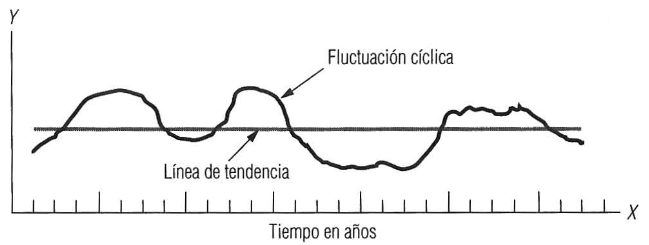
\includegraphics[width=0.7\textwidth]{pictures/tsc3.png}
    \caption{Representación de Variación cíclica en una serie de tiempo}
    \label{fig:tsc3}
  \end{figure}
  
  \item{\textbf{Variación Irregular}}: se debe a factores a corto plazo, imprevisibles y no recurrentes que afectan a la serie de tiempo. Como este componente
  explica la variabilidad aleatoria de la serie, es impredecible; no se puede esperar predecir su impacto sobre la serie de tiempo. Existen dos tipos 
  de variación irregular: a) Las variaciones que son provocadas por acontecimientos especiales, fácilmente identificables, como las elecciones, inundaciones,
  huelgas, terremotos. b) Variaciones aleatorias o por casualidad, cuyas causas no se pueden señalar en forma exacta, pero que tienden a equilibrarse a la larga.
  \begin{figure}[htb]
    \centering 
    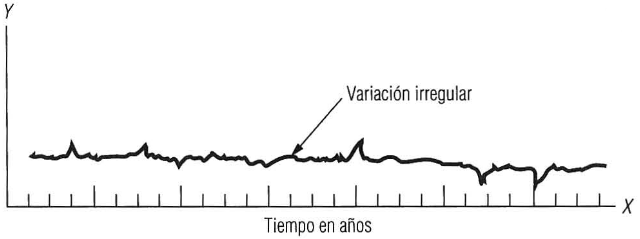
\includegraphics[width=0.7\textwidth]{pictures/tsc4.png}
    \caption{Representación de Variación Irregular en una serie de tiempo}
    \label{fig:tsc4}
  \end{figure}

\end{itemize}

%http://www.scielo.org.co/scielo.php?pid=S0121-47722008000100007&script=sci_arttext&tlng=pt

\subsection{Análisis Grafico de una Serie de Tiempo}

Por muy simple que parezca, el paso más importante en el análisis de series de tiempo consiste en graficar la serie, esto debe hacerse siempre, independiente de cuán 
simples o complejos sean los procedimientos que se emplean posteriormente. El análisis del gráfico de la serie permitirá detectar los siguientes elementos: 
\begin{itemize}
 \item{\textbf {Outliers:}} representa cambios abruptos en los puntos de la serie que se escapan de lo normal; si una serie temporal tiene observaciones anormalmente elevadas 
  (o reducidas), y no se tratan de modo especial, podrían dominar los resultados obtenidos de la estimación. A modo de intuición recuérdese que MCO minimiza la suma de
  cuadrados de los residuos, y el cuadrado del residuo de estos valores será anormalmente alto. Por lo tanto, el estimador tenderá a sobreponderar estos valores
  anómalos, afectando a los parámetros estimados y reduciendo el ajuste total del modelo. La aparición de un outlier puede tener un motivo identificable, en algunas 
  ocasiones no es sencillo encontrar la causa que provoca el outlier. Se trata de casos en los que es probable que el outlier se deba a algún error en el proceso de 
  tratamiento de la información.
  
  Un adecuado tratamiento para contrarestar los efectos del outlier es sustituirlo por una media móvil ponderada ad-hoc de los valores cercanos, aunque esta solución no es 
  eficiente debido a que puede descarta información relevante. Otra medida muy utilizada es la de incorporar el outlier en el modelo por medio de variables ficticias, para 
  controlar su efecto.
  \begin{figure}[htb]
    \centering 
    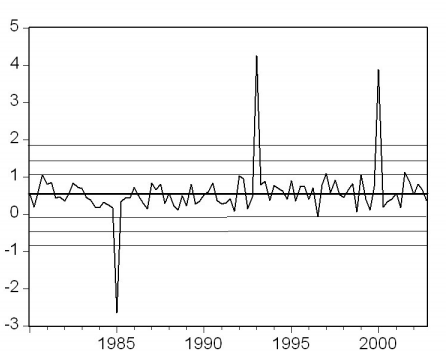
\includegraphics[width=0.55\textwidth]{pictures/outlier.png}
    \caption{Representación de Outliers en una serie de tiempo}
    \label{fig:outlier}
  \end{figure}
  \item{\textbf{Tendencias:}} La tendencia representa el comportamiento predominante de la serie, se puede definir como un cambio a largo plazo que se produce en relación 
  al nivel medio, o el cambio a largo plazo de la media. La tendencia se identifica con un movimiento suave de la serie a largo plazo. 
  Una forma de visualizar la tendencia es mediante suavizamiento de la serie, la idea central es definir a partir de la serie observada una nueva serie que filtra o suaviza
  los efectos ajenos a la tendencia (estacionalidad, efectos aleatorios), de manera que podamos visualizar la tendencia. 
  \begin{figure}[htb]
    \centering 
    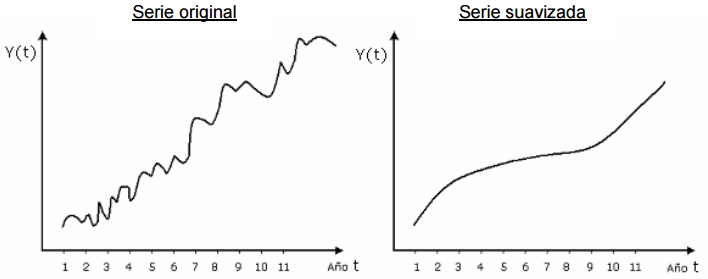
\includegraphics[width=0.55\textwidth]{pictures/tendence.png}
    \caption{Tendencia luego de suavizamiento de una serie de timepo}
    \label{fig:tendence}
  \end{figure}
\end{itemize}
El gráfico de una serie de tiempo permite visualizar de mejor forma los componentes de una serie de tiempo, facilitando un análisis mediante la percepción visual y resumiendo
el comportamiento de un evento a lo largo del registro de sus observaciones.

\subsection{Suavizar la Serie de Tiempo}
Los métodos de suavizamiento contrarestan a las fluctuaciones aleatorias causadas por el componente irregular de la serie. Estos métodos resultan apropiados para series 
estables, es decir, aquellas que no exhiban ningún comportamiento de tendencia, ni variaciones cíclicas ni estacionales, además es conveniente suavizar cuando existen 
cambios bruscos o movimientos irregulares en la serie. A continuación se detalla los métodos más comunes utilizados para suavizar una serie de tiempo.
\begin{itemize}
 \item{\textbf{Método de Medias Móviles:}} El objetivo es eliminar de la serie los componentes estaciónales y accidentales; utiliza como pronóstico para el siguiente período,
 el promedio de los $n$ valores de los datos más recientes de la serie de tiempo, matemáticamente puede expresarse como:
 \begin{equation}
  Promedio Movil=\frac{\sum (n\ valores\ de\ datos\ más\ recientes)}{n} 
 \end{equation}
  El término móvil indica que conforme se tenga disponible una nueva observación de la serie de tiempo, se reemplaza la observación más antigua en la ecuación y se calcula un
  nuevo pronóstico. Como resultado el promedio se modificará, a medida que se agreguen nuevas observaciones.

  La variable $n$ es una indicación de cuantos períodos habrán que tomarse para calcular el promedio, generalmente suele variar entre 3 a 5, dependiendo de cuantos elementos 
  tiene la serie de datos. Para eliminar el componente irregular o el componente estacional en la construcción de una serie de variables a partir de los datos originales se 
  aplica las variaciones del método listadas a continuación.
  \begin{itemize} 
   \item Media móvil anual o de orden 12: Consiste en sustituir el dato de cada mes por el promedio de los datos de los últimos 12 meses, es decir: 
    \begin{equation}
      M_t^{12}=\frac{\sum_{t=1}^{12} y_{t-1}}{12} 
    \end{equation}
   \item Para una Serie Mensual con Estacionalidad Anual $(s=12)$
    \begin{equation}
      \scriptsize{ y(k)=\frac{\frac{1}{2}y(k-6)+ y(k-5)+...+y(k+5)+\frac{1}{2}y(k+6)}{12}}\ ,\ tal\ que\ 7 \leq k \leq n-6)
    \end{equation}
   \item Para una serie trimestral, con estacionalidad anual$(s=4)$
    \begin{equation}
      \scriptsize{ y(k)=\frac{\frac{1}{2}y(k-2)+ y(k-1)+y(k)+y(k+1)+\frac{1}{2}y(k+2)}{4}}\ ,\ tal\ que\ 3 \leq k \leq n-2)
    \end{equation}
    A este procedimiento se le llama: filtro simétrico finito.
   \item Media Móvil de Orden $s$:  Podemos construir medias móviles de orden inferior a 12, es decir, que no sean anuales. Así, la Media Móvil de Orden 3 se construye 
    promediando los tres últimos datos. De manera general, la Media Móvil de Orden $s$ se construye de la siguiente forma:
    \begin{equation}
      M_t^{s}=\frac{y_1+y_{t-1}+y_{t-2+...++y_{t-s+1}}}{s} 
    \end{equation}
    La principal ventaja que presenta esta media móvil será que no retrasará tanto la evolución de la variable como lo hacía la media móvil anual, ya que al no utilizar 
    tantas observaciones, su comportamiento se asemejará más al de la serie original. Sin embargo, el principal inconveniente de esta media móvil viene precisamente de esa 
    menor utilización de observaciones. Al no construirse con 12 observaciones, no se elimina completamente el componente estacional, llegando en ciertos casos a 
    multiplicarse este efecto.
   \item Media Móvil Centrada: Esta media móvil no se construye promediando los datos anteriores al dato original, sino que se utilizan simétricamente los datos adyacentes. 
    En general, la Media Móvil Centrada de orden $s$ va a estar definida por la siguiente expresión:
    \begin{equation}
      \scriptsize{ MC_1^s=\frac{Y_{t+\frac{s-1}{2}}+...y_{t+1}+y_1+y_{t-1}+...+y_{t-\frac{s-1}{2}}}{s}}
    \end{equation}
    La principal ventaja de esta media móvil es que al utilizar los datos adyacentes, tanto anteriores como posteriores, no vamos a tener el problema de retrasar la evolución
    de la variable, es decir, tanto la serie original como la media móvil centrada van a tener en las mismas fechas los valores máximos y mínimos. El principal inconveniente 
    será que al utilizar las observaciones posteriores a cada dato original, para su construcción, no tendremos observaciones de la MC al final de la muestra disponible, 
    siendo ésta precisamente la parte de la muestra más interesante para el análisis. Esta dificultad se resuelve si disponemos de predicciones fiables para los próximos meses.
  \end{itemize}
  \item{\textbf{Método de Suavización Exponencial Simple:}} Esta técnica se basa en la atenuación de los valores de la serie de tiempo, obteniendo el promedio de estos de 
  manera exponencial; es decir, los datos se ponderan dando un mayor peso a las observaciones más recientes y uno menor a las más antiguas. Al peso para ponderar la 
  observación más reciente se le da el valor $\alpha $, la observación inmediata anterior se pondera con un peso de a $(1 - \alpha )$, a la siguiente observación inmediata anterior 
  se le da un peso de ponderación de a $(1 - \alpha )^2$ y así sucesivamente hasta completar el número de valores observados en la serie de tiempo a tomar en cuenta para realizar 
  la atenuación, es decir, para calcular el promedio ponderado. La estimación o pronóstico será el valor obtenido del cálculo del promedio. Por lo que la expresión para realizar 
  el cálculo de la suavización exponencial simple es:
  \begin{equation}
      P_{t+1}=\alpha Y_1 + \alpha ( \alpha -1)Y_{t-1}+\alpha ( \alpha -1)^2Y_{t-2}+... \alpha ( \alpha -1)^{n-1}Y_{t-(n-1)}      
  \end{equation}
  $Donde\\ Y_t: Valor de la serie en el período t.\\ P_{t+1}: Pronóstico o predicción para el período t+1\\ \alpha : Factor de suavización, ( 0 \leq \alpha  \leq 1 )\\
  $\\
  Es decir el valor de la serie suavizada en el período $t+1$ es igual a $\alpha$ veces el valor de la serie en el período $t$, más $1-\alpha$ veces el valor predicho en el período $t$. Es así 
  que para determinar los valores de la serie suavizada se necesita un valor inicial $P_0$, el cual puede ser un promedio de los datos anteriores o simplemente el primer valor de la serie. 
\end{itemize}


 




\section{Bases de Datos Espacio-Temporales}

Dos campos que han surgido a mediados y finales de la década de 1980 son las bases de datos espaciales y bases de
datos temporales las cuales se han convertido, en cierto modo como las precursoras de las bases de datos
espacio-temporales.


\textbf{Base de datos espaciales} 

Las bases de datos espaciales tratan del eficiente almacenamiento y la recuperación de objetos en
el espacio que tienen identidad y extensión bien definidas, ubicaciones, así como ciertas relaciones geométricas
y / o topológica entre ellas, debido al desarrollo en campos de aplicación ( GIS, diseño VLSI, CAD) que necesita
tratar con grandes cantidades de entidades geométricas, geográficas o espaciales. Además de algunos estables y 
maduros prototipos basado en fundamentos algebraicos de tipo solido,  proveedores de sistemas gestores de bases de
datos comercial (DBMS) han ofrecido extensiones de sus productos, soportando tipos espaciales y operaciones
(Oracle Spatial, DB2 Spatial Extender, PostgresGIS , Microsoft SQL Server, MySQL). Sin lugar a dudas, los 
resultados en bases de datos espaciales han impulsado varias líneas de investigación importantes en bases
de datos de objetos en movimiento (MOD), como por ejemplo: consultas populares de MOD (rango, 
vecino mas cercano), propiedades topológicas y relaciones entre tipos espaciales. \cite{yuzheng2011}


\textbf{Base de datos temporales}


Existen muchas aplicaciones de bases de datos, como por ejemplo, contabilidad, gestión de cartera, registros médicos
y gestión de inventario; información que varia en el tiempo. El centro de las bases de datos temporales se
diferencia por:

\begin{description}
 \item [Tiempo válido de un hecho,] es el tiempo en el cual un dato particular es recogido y se convierte en verdad
 hasta donde el mundo representado por la base de datos es referida, 
posiblemente abarque el pasado, el presente y el futuro. Sin embargo, el tiempo válido no puede ser 
conocido, o los registros no pueden ser relevantes para las aplicaciones soportadas por la base de datos
o en el caso que los modelos de base de datos del mundo real puedan variar entre los diferentes mundos reales.

\item [Tiempo de transacción de un hecho,] es el tiempo que un hecho dado es el actual en la base de datos. 
El tiempo de transacción puede asociarse con diferentes entidades de bases de datos, como, por ejemplo,
objetos y valores que no son hechos, porque no pueden ser verdaderos o falsos en forma aislada. Por lo tanto, todas las entidades de la base de datos tiene un aspecto de tiempo de transacción, que tiene
una duración: desde inserción (lógico) a la eliminación de una determinada entidad.
\end{description}


Capturar el tiempo variable utilizando los modelos de datos tradicionales y lenguajes de consulta
puede ser una actividad engorrosa y, como consecuencia, se necesitan construcciones que permitirán
capturar los tiempos válidos y operación de los hechos, lo que conduce a relaciones temporales. Además,
en los lenguajes de consulta se necesitan extensiones sintácticas que permiten las operaciones de base
de datos en modelos temporales. \cite{yuzheng2011}

\section{Técnicas de Regresión}

Permiten investigar y modelar la relación entre variables, la principal ventaja de la regresión es la descripción de los datos con el 
objetivo de resumir y ajustar un conjunto de datos. Adicionalmente es posible realizar una estimación de parámetros. Una vez 
seleccionado los modelos de regresión es necesario realizar un análisis y comparación de los diferentes modelos de regresión y 
chequear que tan bueno es un modelo ajustado respecto a otro. El resultado de este chequeo puede indicar si el modelo es razonable 
o si el ajuste original debe ser modificado.\\
\textbf{\\Selección de las variables del modelo}\\
Existen varios métodos para construir el modelo de regresión, es decir, para seleccionar de entre todas las variables que introducimos 
en el modelo, cuáles son las que necesitamos para explicarlo. El modelo de regresión se puede construir utilizando las siguientes técnicas \cite{regresionmodel}: 
\begin{itemize}
\item{\textbf{Técnica de pasos hacia adelante (Forward)} 
Consiste en ir introduciendo las variables en el modelo únicamente si cumplen una serie de condiciones hasta que no se pueda introducir 
ninguna más, hasta que ninguna cumpla la condición impuesta
}
\item{
\textbf{Técnica de pasos hacia atrás (Backward)}
Se introducen en el modelo todas las variables y se van suprimiendo si cumplen una serie de condiciones definidas a priori hasta 
que no se pueden eliminar más, es decir ninguna variable cumpla la condición impuesta.
}
\item{\textbf{Técnica por pasos (Stepwise)}
Combina los dos métodos anteriores, adelante y atrás introduciendo o eliminando variables del modelo si cumplen una serie de 
condiciones definidas a priori hasta que ninguna variable satisfaga ninguna de las condiciones expuestas de entrada o salida del modelo.
}
\item{\textbf{Técnica de introducir todas las variables obligatoriamente (Enter)}
Esta última técnica de selección de variables para construir el modelo de regresión, produce que el proceso de selección de las variables 
sea manual, partiendo de un modelo inicial, en el que se obliga a que entren todas las variables seleccionadas, se va evaluando qué variable 
es la que menos participa en él y se elimina, volviendo a construir un nuevo modelo de regresión aplicando la misma técnica, pero excluyendo 
la variable seleccionada y aplicando el mismo proceso de selección. Este proceso se repite reiteradamente hasta que se considere que el modelo 
obtenido es el que mejor se ajusta a las condiciones impuestas y que no se puede eliminar ninguna variable más de las que los componen.
}
\end{itemize}
\section{Redes Neuronales}
Se define redes neuronales a una nueva forma de computación inspirada en modelos biológicos, un modelo matemático compuesto
por un gran número de elementos procesales organizados en niveles, también se define redes neuronales a un sistema de computación compuesto 
por un gran número de elementos simples, elementos de procesos muy interconectados, los cuales procesan información por medio de su estado dinámico 
como respuesta a entradas externas o se puede definir las redes neuronales como redes interconectadas masivamente en paralelo de elementos simples y 
con organización jerárquica, las cuales intentan interactuar con los objetos del mundo real del mismo modo que lo hace el sistema nervioso 
biológicos~\ref{fig:rn}.
\begin{figure}[htb]
 \centering 
 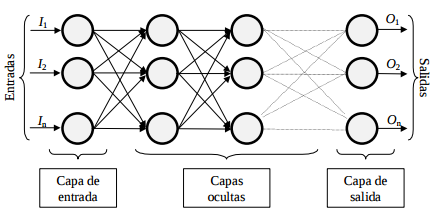
\includegraphics[scale=0.7]{pictures/rn.png}
 \caption{ un esquema de una red neuronal.} 
 \label{fig:rn}
\end{figure}
\newpage
Las redes neuronales presentan características como:
\begin{itemize}
 \item {\textbf{ Aprendizaje adaptativo}\\
 Las redes neuronales pueden aprender a diferenciar patrones mediante ejemplos y entrenamientos, no es necesario elaborar modelos a priori 
 ni necesidad de especificar funciones de distribución de probabilidad; las RN son sistemas dinámicos auto-adaptativos con la capacidad de 
 auto-ajuste de los elementos procesales (neuronas) que componen el sistema, son capaces de estar constantemente
cambiando para adaptarse a las nuevas condiciones; los enlaces ponderados de las neuronas se ajustan de manera que se obtengan ciertos 
resultados específicos. Una red neuronal no necesita un algoritmo para resolver un problema, ya que ella puede generar su propia distribución
de pesos en los enlaces mediante el aprendizaje. También existen redes que continúan aprendiendo a lo largo de su vida, después de completado 
su período de entrenamiento.
 }
\item {\textbf{ Auto-organización }\\
 Las redes neuronales emplean su capacidad de aprendizaje adaptativo para auto-organizar la información que reciben durante el aprendizaje 
 y/o la operación. Mientras que el aprendizaje es la modificación de cada elemento procesal, la auto-organización consiste en la modificación
 de la red neuronal completa para llevar a cabo un objetivo específico.
Cuando las redes neuronales se usan para reconocer ciertas clases de patrones,
ellas auto-organizan la información usada. Por ejemplo, la red llamada backpropagation,
creará su propia representación característica, mediante la cual puede reconocer ciertos
patrones.Esta auto-organización provoca la generalización: facultad de las redes
neuronales de responder apropiadamente cuando se les presentan datos o situaciones a
las que no había sido expuesta anteriormente. El sistema puede generalizar la entrada
para obtener una respuesta. 

Esta característica es muy importante cuando se tiene que
solucionar problemas en los cuales la información de entrada no es muy clara; además
permite que el sistema dé una solución, incluso cuando la información de entrada está
especificada de forma incompleta. 
 } 
 \item {\textbf{ Tolerancia a fallos }\\
 Las redes neuronales fueron los primeros métodos computacionales con la capacidad inherente de tolerancia a fallos. Comparados con los sistemas 
 computacionales tradicionales, los cuales pierden su funcionalidad cuando sufren un pequeño error de memoria, en las redes neuronales, si se 
 produce un fallo en un número no muy grande de neuronas y aunque el comportamiento del sistema se ve influenciado, no sufre una caída repentina.
Hay dos aspectos distintos respecto a la tolerancia a fallos:
\begin{itemize}
\item Las redes pueden aprender a reconocer patrones con ruido, distorsionados o
incompletos. Esta es una tolerancia a fallos respecto a los datos.
\item Las redes pueden seguir realizando su función (con cierta degradación)
aunque se destruya parte de la red.
\end{itemize}
La razón por la que las redes neuronales son tolerantes a los fallos es que tienen
su información distribuida en las conexiones entre neuronas, existiendo cierto grado de
redundancia en este tipo de almacenamiento. La mayoría de los ordenadores
algorítmicos y sistemas de recuperación de datos almacenan cada pieza de información
en un espacio único, localizado y direccionable. En cambio, las redes neuronales
almacenan información no localizada. Por lo tanto, la mayoría de las interconexiones
entre los nodos de la red tendrán sus valores en función de los estímulos recibidos, y se
generará un patrón de salida que represente la información almacenada. 
 } 
 \item {\textbf{ Operación en tiempo real }\\
 Una de las mayores prioridades, casi en la totalidad de las áreas de aplicación, es
la necesidad de realizar procesos con datos de forma muy rápida. Las redes neuronales
se adaptan bien a esto debido a su implementación paralela. Para que la mayoría de las
redes puedan operar en un entorno de tiempo real, la necesidad de cambio en los pesos
de las conexiones o entrenamiento es mínimo.
 } 
 \item {\textbf{ Fácil inserción dentro de la tecnología existente. }\\
 Una red individual puede ser entrenada para desarrollar una única y bien
definida tarea (tareas complejas, que hagan múltiples selecciones de patrones,
requerirán sistemas de redes interconectadas). Con las herramientas computacionales
existentes (no del tipo PC), una red puede ser rápidamente entrenada,
comprobada, verificada y trasladada a una implementación hardware de bajo
coste. Por lo tanto, no se presentan dificultades para la inserción de redes
neuronales en aplicaciones específicas, por ejemplo de control, dentro de los
sistemas existentes. De esta manera, las redes neuronales se pueden utilizar para
mejorar sistemas en forma incremental y cada paso puede ser evaluado antes de
acometer un desarrollo más amplio \cite{pitarque2000redes}.
 }
\end{itemize}

Entre las propiedades de las RN que han llamado la atención de los estadísticos destacan las relativas a su buen rendimiento ante
problemas no lineales o datos con mucho «ruido», y el poderse utilizar independientemente del cumplimiento de los supuestos teóricos 
relativos a las técnicas estadísticas (y de ahí que se haya hablado de ellas como de «técnicas de distribución libre o no paramétricas»). 
Por ello las RN han sido aplicadas a problemas de tradición estadística como predicción y clasificación (a través de las
llamadas redes hetero-asociativas: perceptrón multicapa y redes de función base radial), reducción de la dimensionalidad (a través
de las llamadas redes auto-asociativas: Hopfield, Kohonen),series temporales, etc.\cite{pitarque1998redes}\cite{maneta2003aplicacion}\cite{rn2001giaiq}.

\section{Interpolación Espacial}

La interpolación espacial es el proceso de utilizar puntos con valores conocidos para estimar valores desconocidos en otros puntos. 
Por ejemplo, para realizar un mapa de precipitación (lluvia) para el país no se encontrarán suficientes estaciones meteorológicas distribuidas
uniformemente para cubrir toda la región. La interpolación espacial puede estimar las temperaturas en lugares que no tienen ese dato utilizando 
lecturas de temperatura conocida en estaciones meteorológicas cercanas~\ref{fig:is}. A este tipo de superficie interpolada con 
frecuencia se le llama una superficie estadística. Datos de elevación, precipitación, acumulación de nieve, tabla de agua y densidad de población 
son otros tipos de datos que pueden ser calculados utilizando la interpolación \cite{qgis2015online}.

Debido al alto costo y a los recursos limitados la recolección de los datos usualmente es llevada a cabo sólo en un número limitado 
de ubicaciones de puntos seleccionados. En un SIG, la interpolación de esos puntos puede ser aplicada para crear una superficie raster con 
estimaciones realizadas para todas las celdas del raster. Con el fin de generar un mapa continuo, por ejemplo, un mapa de elevaciones digitales de 
los puntos de elevación medidos con un dispositivo GPS, se debe utilizar un método de interpolación adecuado para estimar de manera óptima los valores 
en aquellas ubicaciones en donde no fueron tomadas muestras o mediciones. Los resultados del análisis de interpolación pueden entonces ser utilizados 
para análisis que cubran el área completa y para el modelado.

\begin{figure}[htbp]
 \centering 
 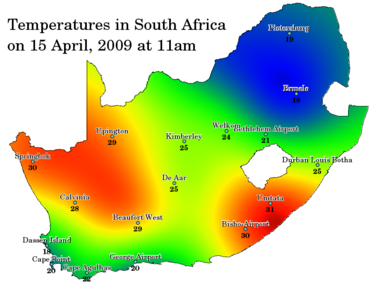
\includegraphics[width=0.6\textwidth]{pictures/is.png}
 \caption{Mapa de temperaturas interpolado de estaciones.}
 \label{fig:is}
\end{figure}
\textbf{Metodos de Interpolación}\bigskip

\textbf{Método Trend Surface}: es un método analítico, global e inexacto a partir de puntos. Este
método se utiliza para separar y describir determinados componentes de variación presentes
en los datos, facilitando su interpretación, puesto que cada una de las observaciones puede ser
considerada como resultado de la adición de un componente regional o de tendencia y un
componente local. Asimismo, considera la autocorelación de la variable.
Ajustándose la variable Z a una ecuación de regresión cuyas variables explicativas son X e Y
de los puntos muestrales. Proporciona una descripción sintética de la superficie ondulada que
se está tratando y de la variación espacial de la variable temática, facilitando un método para
estimar el valor de Z en un punto no muestral cuyas coordenadas X e Y sean conocidas Figura~\ref{fig:m1}.
\begin{figure}[htb]
 \centering 
 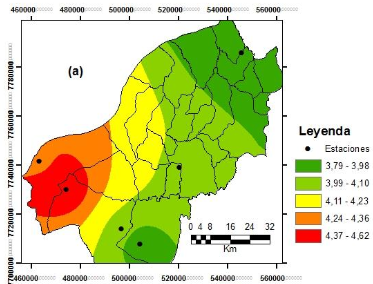
\includegraphics[width=0.47\textwidth]{pictures/a.png}
 \caption{Interpolación con el método Trend Surface\cite{models2013}}
 \label{fig:m1}
\end{figure}

\textbf{Método Moving average}: es un método directo, local, a partir de puntos, puede ser exacto
o no según el factor de ponderación. Se aplica para un gran conjunto de datos. Extrae
tendencias intermedias de un número mínimo de puntos definidos dentro de una Search
Elipse, asociada a cada uno de los puntos del grid. El valor final de cada uno de los puntos del
grid es igual a la media aritmética de todos los puntos vecinos identificados. Si dentro de la
Search elipse no hay un número mínimo de puntos definidos para el cálculo, el área estará en
blanco Figura~\ref{fig:m2}.
\begin{figure}[htb]
 \centering 
 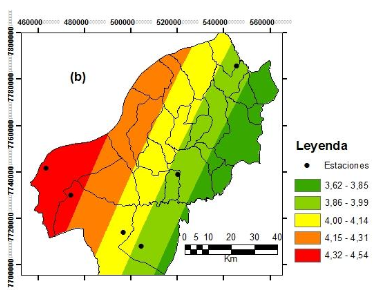
\includegraphics[width=0.47\textwidth]{pictures/b.png}
 \caption{Interpolación con el método Moving Average\cite{models2013}}
 \label{fig:m2}
\end{figure}

\textbf{Método Kriging}: es un método analítico, donde la función de interpolación depende de la
autocorelación espacial de la variable, que se representa en variogramas. Utiliza datos
tabulares y su posición geográfica para el cálculo de las interpolaciones. Utilizando el
principio de la primera ley geográfica de Tobler, que dice que las unidades de análisis más
próximas entre si son mas similares que las unidades más lejanas, el kriging utiliza funciones
matemáticas para añadir más peso en las posiciones más cercanas a los puntos de muestreo y
menores pesos en posiciones más distantes, y así crear nuevos puntos interpolados basados en
estas combinaciones lineares de datos. Además se está basado en optimizar funciones usando
autocorelación espacial Figura~\ref{fig:m3}.
\begin{figure}[htb]
 \centering 
 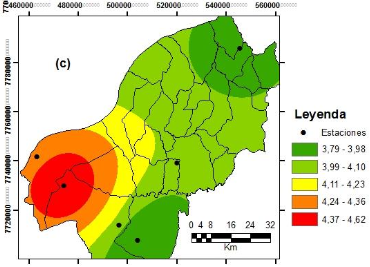
\includegraphics[width=0.5\textwidth]{pictures/c.png}
 \caption{Interpolación con el método Kriging \cite{models2013}}
 \label{fig:m3}
\end{figure}

\section{Minería de Datos}
El descubrimiento de conocimiento en bases de datos (KDD) se define como el proceso de identificar patrones significativos 
en los datos que sean válidos, novedosos, potencialmente útiles y comprensibles para un usuario. El proceso global consiste 
en transformar información de bajo nivel en conocimiento de alto nivel \cite{riquelme2006mineria}. El proceso KDD es interactivo e iterativo conteniendo
los siguientes pasos:
\begin{enumerate}
 \item \textbf{Comprender el dominio de aplicación:} este paso incluye el conocimiento relevante previo y las metas de la aplicación.
\item \textbf{Extraer la base de datos objetivo:} recogida de los datos, evaluar la calidad de los datos y utilizar análisis exploratorio de los datos para
familiarizarse con ellos.
\item \textbf{Preparar los datos:} incluye limpieza, transformación, integración y reducción de datos. Se intenta mejorar la calidad de los
datos a la vez que disminuir el tiempo requerido por el algoritmo de aprendizaje aplicado posteriormente.
\item \textbf{Minería de datos:} como se ha señalado anteriormente, este es la fase fundamental del proceso. Está constituido por una o más de
las siguientes funciones, clasificación, regresión, clustering, resumen, recuperación de imágenes, extracción de reglas, etc.
\item \textbf{Interpretación:} explicar los patrones descubiertos, así como la posibilidad de visualizarlos.
\end{enumerate}
A continuación se comentan brevemente las tareas más comunes en cualquier proceso de la minería de datos.
\begin{itemize}
 \item Clasificación: clasifica un dato dentro de una de las clases categóricas predefinidas. Responde a preguntas tales como, 
 ¿Cuál es el riesgo de conceder un crédito a este cliente? ¿Dado este nuevo paciente qué estado de la enfermedad indican sus análisis?
 \item Regresión: el propósito de este modelo es hacer corresponder un dato con un valor real de una variable. Responde a cuestiones como
¿Cuál es la previsión de ventas para el mes que viene? ¿De qué depende?
 \item Clustering: se refiere a la agrupación de registros, observaciones, o casos en clases de objetos similares. Un cluster es una colección
de registros que son similares entre sí, y distintos a los registros de otro cluster. ¿Cuántos tipos de clientes vienen a mi negocio? 
¿Qué perfiles de necesidades se dan en un cierto grupo de pacientes?
\item Generación de reglas: aquí se extraen o generan reglas de los datos. Estas reglas hacen referencia al descubrimiento de relaciones de 
asociación y dependencias funcionales entre los diferentes atributos.
\item Resumen o sumarización: estos modelos proporcionan una descripción compacta de un subconjunto de datos. ¿Cuáles son las
principales características de los datos?
\item Análisis de secuencias: se modelan patrones secuenciales, como análisis de series temporales, secuencias de genes, etc. El objetivo 
es modelar los estados del proceso, o extraer e informar de la desviación y tendencias en el tiempo. ¿El consumo de energía eléctrica de este 
mes es similar al del año pasado? Dados los niveles de contaminación atmosférica de la última semana cuál es la previsión para las próximas 24 horas.
\end{itemize}


\textbf{Patrones Frecuentes en Bases de Datos Tradicionales}

Patrones frecuentes son conjuntos de elementos, subsecuencias, o subestructuras que aparecen en un conjunto de datos con una
frecuencia no inferior a un umbral especificado por el usuario \cite{han2007frequent}. La cuestión de las modalidades 
interesantes desvelando en las bases de datos en diferentes contextos ha sido un tema de investigación
recurrente durante los últimos 15 años. Minería de datos general ha sido ampliamente reconocido como un
crítico campo por empresas de todo tipo. Como parte de los métodos de minería de datos, la tarea de aprendizaje 
de reglas de asociación han estudiado diferentes algoritmos de minería de patrones frecuente de identificar 
tendencias relevantes en los conjuntos de datos en diferentes disciplinas \cite{creighton2003mining}. 

Una de las áreas en las que las técnicas de aprendizaje de reglas de asociación y el patrón frecuente 
algoritmos de minería se han aplicado con más frecuencia en el análisis de datos y tendencias del
mercado en transacciones de clientes de grandes supermercados y tiendas \cite{agrawal1994fast}. Por lo general, esta técnica 
tiene dado el nombre del problema de la cesta de compras a pesar de que los métodos derivados de resolverlo
puede ser aplicado en diferentes contextos \cite{han2006data}.

\textbf{Minería de Patrones Secuenciales}

Sea DB un conjunto de registros (objetos), donde cada registro R consiste de tres
elementos de información:
\begin{itemize}
\item un identificador de registro object-id
\item un registro de tiempo timestamp
\item un conjunto A de atributos binarios
\end{itemize}
Un atributo a puede estar presente ’1’, o ausente ’0’. Si bien los algoritmos intentan encontrar secuencias de atributos
presentes, esta claro que su ausencia también brinda significativa información. Un atributo a presente es llamado
ítem i, y dentro del contexto de números, un ítem es una cupla (atributo, valor). Un conjunto de items
{i1, i2, · · · , ik} es denotado por I, donde I es un sub conjunto de A. Esto es una representación no ordenada. Una
secuencia s es una lista ordenada no vacía de los conjuntos de items s, denotado por hs1, s2, · · · , spi. Una nsecuencia
es una secuencia de n items o de tamaño n. Decimos entonces que R es un conjunto de registros que
contienen los atributo presente (o ítems) i. Gráficamente R(I) podría verse así como en la figura ~\ref{fig:atrib}.

\begin{figure}[htb]
 \centering 
 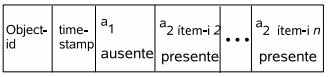
\includegraphics[scale=0.5]{pictures/atrib.png}
 \caption{Algunos Atributos Presentes o items.} 
 \label{fig:atrib}
\end{figure}

\textbf{Secuencia de datos} Una secuencia de datos hs1, s2, · · · , spi es una agrupación
ordenada de registros con atributos presentes iguales, similares o pertenecientes. La agrupación se ordena según los
datos de timestamp. \\
\textbf{Frecuencia de secuencias} Los grados de pertenencia se obtienen al evaluar la frecuencia
de ocurrencia de las secuencias freq(s) con distintos niveles. Algunos autores establecen un valor
de referencia o parámetro, por ejemplo minFreq, con el fin de decidir si una frecuencia es más o menos frecuente.\\

\textbf{LCM (Linear Time Closed Itemset Miner)}

El problema de LCM propuesto por \cite{uno2005lcm} se define de la siguiente manera.
Sea I un conjunto de elementos. Sea D una base de datos transaccional de tal manera que cada 
registro (llamada transacción) es un conjunto de elementos. La frecuencia de un conjunto de 
elementos es el número de transacciones, incluyendo el conjunto de elementos. Para un número dado t 
(llamado soporte), un conjunto de elementos se dice que es frecuente si su frecuencia es no menos de 
t. Un conjunto de elementos frecuente se llama máxima si está incluido en ningún otro conjunto de 
elementos frecuentes, y se llama cerrada si está incluido en ningún otro conjunto de elementos de la 
misma frecuencia. La tarea de LCM, es enumerar (sacar, o contar) todos los conjuntos de elementos 
frecuentes, todos los conjuntos de elementos frecuentes máximos, o todos los conjuntos de elementos 
frecuentes cerrados en una base de datos transaccional para un soporte dado.